\documentclass[11pt]{exam}
\newcommand{\myname}{Nishant Aswani}
\newcommand{\mynetid}{nsa325}
\newcommand{\myemail}{nsa325@nyu.edu}
\newcommand{\myhwtype}{Homework}
%%%%%%%%%%%%%%%%%%%%%%%%%%%%%%%%
\newcommand{\myhwnum}{11}
%%%%%%%%%%%%%%%%%%%%%%%%%%%%%%%%
\newcommand{\mycoursenumber}{ENGR-UH 3511}
\newcommand{\myclassname}{Computer Organization and Architecture}

\newcommand{\cc}[1]{\texttt{#1}}

% Prefix for numedquestion's
\newcommand{\questiontype}{Question}

% Use this if your "written" questions are all under one section
% For example, if the homework handout has Section 5: Written Questions
% and all questions are 5.1, 5.2, 5.3, etc. set this to 5
% Use for 0 no prefix. Redefine as needed per-question.
\newcommand{\writtensection}{0}

\usepackage{amsmath, amsfonts, amsthm, amssymb}  % Some math symbols
\usepackage{enumerate}
\usepackage{enumitem}
\usepackage{graphicx}
\usepackage{hyperref}
\usepackage[all]{xy}
\usepackage{wrapfig}
\usepackage{fancyvrb}
\usepackage[T1]{fontenc}
\usepackage{listings}
\lstset{
  basicstyle=\ttfamily,
  mathescape
}
\usepackage{fancyhdr}
\usepackage{booktabs}
\usepackage{makecell}
\usepackage{hhline}
\usepackage[utf8]{inputenc}

\usepackage[sorting=none,style=numeric]{biblatex}
\addbibresource{refs.bib}

% \usepackage{centernot}
\usepackage{mathtools}
\DeclarePairedDelimiter{\ceil}{\lceil}{\rceil}
\DeclarePairedDelimiter{\floor}{\lfloor}{\rfloor}
\DeclarePairedDelimiter{\card}{\vert}{\vert}

% Uncomment the following line to get Solarized-themed source listings
% You will have had to already installed the solarized-light package
% https://github.com/jez/latex-solarized
%
%\usepackage{solarized-light}

\setlength{\parindent}{0pt}
\setlength{\parskip}{5pt plus 1pt}
\pagestyle{empty}

\def\indented#1{\list{}{}\item[]}
\let\indented=\endlist

\newcounter{questionCounter}
\newcounter{partCounter}[questionCounter]

\newenvironment{namedquestion}[1]{%
    \addtocounter{questionCounter}{1}%
    \setcounter{partCounter}{0}%
    \vspace{.2in}%
        \noindent{\bf #1}%
    \vspace{0.3em} \hrule \vspace{.1in}%
}{}

\newenvironment{numedquestion}[0]{%
	\stepcounter{questionCounter}%
    \vspace{.2in}%
        \ifx\writtensection\undefined
        \noindent{\bf \questiontype \; \arabic{questionCounter}. }%
        \else
          \if\writtensection0
          \noindent{\bf \questiontype \; \arabic{questionCounter}. }%
          \else
          \noindent{\bf \questiontype \; \writtensection.\arabic{questionCounter} }%
        \fi
    \vspace{0.3em} \hrule \vspace{.1in}%
}{}

\newenvironment{alphaparts}[0]{%
  \begin{enumerate}[label=\textbf{(\alph*)}]
}{\end{enumerate}}

\newenvironment{arabicparts}[0]{%
  \begin{enumerate}[label=\textbf{\arabic{questionCounter}.\arabic*})]
}{\end{enumerate}}

\newenvironment{questionpart}[0]{%
  \item
}{}

\newcommand{\answerbox}[1]{
\begin{framed}
\vspace{#1}
\end{framed}}

\pagestyle{head}

\headrule
\header{\textbf{NYU Abu Dhabi}}%
{\textbf{}}%
{\textbf{Division of Engineering}}

\pagestyle{head}

\begin{document}

\begin{center}
  
\includegraphics[scale=0.15]{etc/NYUAD-alt-logo.jpg}
\end{center}

{\vspace{1.5em}}

\begin{center}
    \Huge{\textbf{\mycoursenumber}}\\
    {\vspace{0.5em}}
    \Huge{\textbf{\myclassname}}
\end{center}

{\vspace{10em}}

\begin{center}
  \begin{tabular}{|rp{5.0cm}lll|}
    \hline
    &  &  &  & \\
    &  &  &  & \\
    \Large{\textbf{Name:}} & \Large{\myname}
    
    \  &  &  & \\
    \Large{\textbf{Net ID:}} & \Large{\mynetid}
    
    \  &  &  & \\
    \Large{\textbf{Assignment Title:}} & \Large{\myhwtype{} \myhwnum}
    
    \
    
    \  &  &  & \\
    \hline
  \end{tabular}
\end{center}

\

{\newpage}


\thispagestyle{plain}
\begin{center}
  {\Large \mycoursenumber{} \myhwtype{} \myhwnum} \\
  \myname{} (\myemail{}) \\
  \today
\end{center}

\setcounter{questionCounter}{0}

\begin{namedquestion}{Case 4.13}
Assume a GPU architecture that contains 10 SIMD processors. Each SIMD instruction has a width of 32 and each SIMD processor contains 8 lanes for single-precision arithmetic and load/store instructions, meaning that each nondiverged SIMD instruction can produce 32 results every 4 cycles. Assume a kernel that has divergent branches that causes, on average, 80\% of threads to be active. Assume that 70\% of all SIMD instructions executed are single-precision arithmetic and 20\% are load/store. Because not all memory latencies are covered, assume an average SIMD instruction issue rate of 0.85. Assume that the GPU has a clock speed of 1.5 GHz. 
\end{namedquestion}

\begin{namedquestion}{Problem 4.13a}
Compute the throughput, in GFLOP/s, for this kernel on this GPU. 

To begin with we can consider the clock rate, the number of processors, and the number of lanes: 

1.5 GHz $\times$ 10 processors $\times$ 8 lanes

However, at a given time only $80\%$ are active. Moreover, only $70\%$ of these instructions are non-load/store operations. 

1.5 GHz $\times$ 10 processors $\times$ 8 lanes $\times$ 0.8 $\times$ 0.7

So fare we have assumed one instruction per cycle, but because of the memory latencies we must multiply by the issue rate. Hence:

1.5 GHz $\times$ 10 processors $\times$ 8 lanes $\times$ 0.8 $\times$ 0.7 $\times$ 0.85 = 57.12 $\frac{GFLOPs}{sec}$

Dimensional Analysis to confirm: 

$\frac{G cycles}{sec} \times \frac{operations}{cycle} = \frac{G operations}{sec}$  

\end{namedquestion}

\begin{namedquestion}{Problem 4.13b}
Speedup = $\frac{\text{New Throughput}}{\text{Old Throughput}}$\\

(1) To get the new throughput after increasing the number of lanes to 16, we simply multiply the old throughput by 2 obtain the new throughput = 114.24$\frac{GFLOPs}{sec}$. 

Speedup = $\frac{114.24}{57.12} = 2$\\

(2) To get the new throughput using 15 SIMD processors instead of 10, we simply multiply the old throughput by 1.5 to get the new throughput = 85.68$\frac{GFLOPs}{sec}$.

Speedup = $\frac{85.68}{57.12} = 1.5$\\

(3) We can recalculate the new throughput with a latency of 0.95. 

1.5 GHz $\times$ 10 processors $\times$ 8 lanes $\times$ 0.8 $\times$ 0.7 $\times$ 0.95 = 63.84 $\frac{GFLOPs}{sec}$

Speedup = $\frac{63.84}{57.12} = 1.11$\\

The best upgrade would be to increase the number of lanes per SIMD processor. 

\end{namedquestion}

\begin{namedquestion}{Problem 4.14a}

Does this code have a loop-carried dependency?

\begin{lstlisting}
for (i=0;i<100;i++){ 
    A[i] = B[2*i+4]; /* S1 */ 
    B[4*i+5] = A[i]; /* S2 */ 
} 
\end{lstlisting}

No, there are no loop-carried dependencies. Each iteration can be calculated without information from the prior iterations.

Graphing the two functions below, we see that they will never intersect. This proves that there is no dependence. \\

\begingroup
    \centering
    \medskip
    %width=\columnwidth
    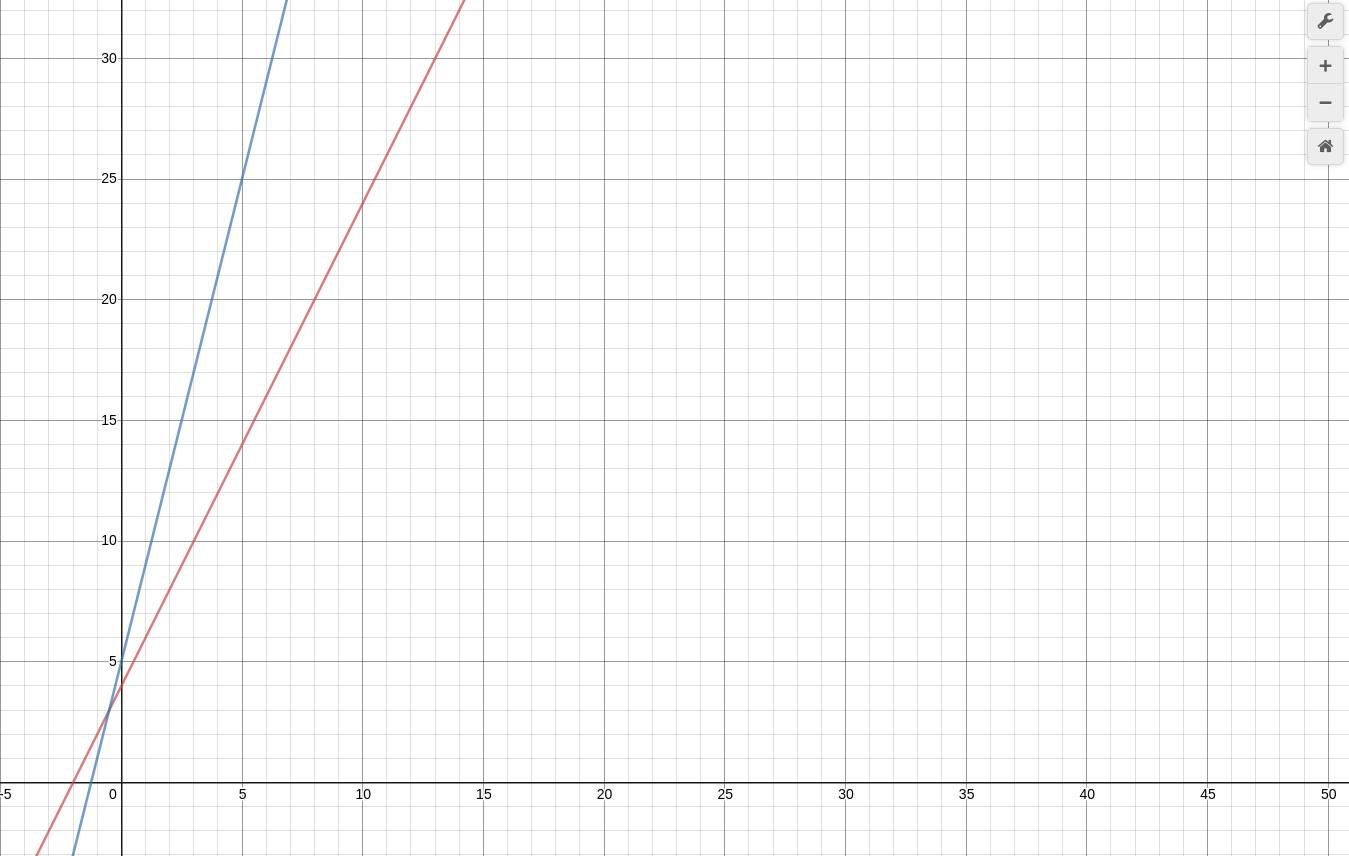
\includegraphics[width=\columnwidth]{Homework-Tex/img/dep.png}
    \medskip
\endgroup

\end{namedquestion}
\newpage
\begin{namedquestion}{Problem 4.14b}

In the following loop, find all the true dependences, output dependences, and antidependences. Eliminate the output dependences and antidependences by renaming. 

\begin{lstlisting}
for (i=0;i <100;i++){
    A[i] = A[i] * B[i]; /* S1 */ 
    B[i] = A[i] + c;    /* S2 */ 
    A[i] = C[i] * c;    /* S3 */ 
    C[i] = D[i] * A[i]; /* S4 */
}
\end{lstlisting}

True dependences:\\
S1 \xrightarrow{t} S2 \\
S3 \xrightarrow{t} S4\\
\\
\text{Output dependences:}\\
S1 \xrightarrow{o} S3 \\
\\
\text{Anti-dependences:}\\
S1 \xrightarrow{a} S2 \\
S1 \xrightarrow{a} S3 \\
S2 \xrightarrow{a} S3 \\
S3 \xrightarrow{a} S4 \\

Renamed (Assume that copies of an array "R" look like "Rx")

\begin{lstlisting}
for (i=0;i <100;i++){
    X[i] = Ax[i] * Bx[i]; /* S1 */ 
    B[i] = X[i] + c;      /* S2 */ 
    A[i] = Cx[i] * c;     /* S3 */ 
    C[i] = D[i] * A[i];   /* S4 */
}
\end{lstlisting}
\end{namedquestion}

\newpage 
\begin{namedquestion}{Problem 4.14c}

Are there dependences between S1 and S2? Is this loop parallel? If not, show how to make it parallel. 

\begin{lstlisting}
for (i=0;i <100;i++){ 
    A[i] = A[i] + B[i];     /* S1 */
    B[i+1] = C[i] + D[i];   /* S2 */ 
} 
\end{lstlisting}

There is a loop-carried true dependence. S2 at iteration i calculates B[i+1] which is used in S1 at iteration i+1. Hence, it is not parallel. \\

The following loop can be parallelized as it seems that the C and D arrays are all precomputed:

\begin{lstlisting}

A[0] = A[0] + B[0]

for (i=1;i <100;i++){ 
    B[i] = C[i-1] + D[i-1]; /* S1 */ 
    A[i] = A[i] + B[i]      /* S2 */ 
} 
\end{lstlisting}





\end{namedquestion}



\printbibliography

\end{document}

% \begingroup
%     \medskip
%     \centering
%     \def\arraystretch{1.5}
%         \begin{tabular}{cc}
%             \toprule
%             RAW hazard & stall cycles\\
%             \midrule
%             Ex to 1st & 2\\
%             Mem to 1st & 2\\
%             Ex to 2nd & 1\\
%             Mem to 2nd & 1\\
%             Ex to 1st and Mem to 2nd & 2\\
%             \bottomrule
%         \end{tabular}
%     \label{fig:c2table2}
%     \medskip
% \endgroup


